\documentclass[oneside,a4paper]{report}
\usepackage{color}
\usepackage{longtable}
\usepackage{titlesec}
\usepackage[hidelinks]{hyperref}
\usepackage{ulem}
\usepackage{graphicx}
\usepackage{fancyhdr}
\usepackage[T1]{fontenc}
\usepackage[headheight=25pt,margin=0.7in,top=1.5in,bottom=1in,right=1in,left=1in]{geometry}

\hypersetup{colorlinks=true,linktoc=none,citecolor=black,urlcolor=blue}
\hypersetup{linktocpage=false,linkcolor=black}

\pagestyle{fancy}
\fancyhead[R]{
\includegraphics[width=2cm]{./latex/resources/kitlogo.png}}
\fancyhead[L]{\leftmark}

\fancypagestyle{plain}{
        \rhead{
\includegraphics[width=2cm]{./latex/resources/kitlogo.png}}
        \lhead{\leftmark}
}


\renewcommand{\arraystretch}{2}

\titleformat{\chapter}[hang]
 {\normalfont\bfseries\LARGE}{\thechapter. }{0pt}{\LARGE}
\titleformat{\section}[hang]
 {\normalfont\bfseries\Large}{\thesection. }{0pt}{\Large}
\titleformat{\paragraph}[hang]
 {\normalfont\bfseries\normalsize}{}{}{}

\titlespacing*{\chapter}{0pt}{-20pt}{10pt}

\begin{document}
  \begin{titlepage}
	\centering
	{\scshape\LARGE Karlsruhe Institute of Technology \par}
	\vspace{1cm}
	{\scshape\Large Software Engineering Practice\par}
	\vspace{0.5cm}
	{\scshape\Large WINTER TERM 2015/2016\par}
	\vspace{1.5cm}
	{\Huge\bfseries rootJS - module guide\par}
	\vspace{0.25cm}
	{\Large\bfseries Node.js bindings for ROOT 6\par}
	\vspace{2cm}
	{\Large\itshape Jonas Schwabe\par}
	{\Large\itshape Theo Beffart\par}
	{\Large\itshape Sachin Rajgopal\par}
	{\Large\itshape Christoph Wolff\par}
	{\Large\itshape Christoph Haas\par}

	{\Large\itshape Maximilian Fr\"uh\par}
	\vfill
	supervised by\par
	Dr.~Marek \textsc{Szuba}

	\vfill

	% Bottom of the page
	{\large \date{99.99.9999}\par}
\end{titlepage}

  \tableofcontents
  \clearpage
\chapter{NodeApplication}
describe class NodeApplication here
\section{NodeApplication}
\begin{longtable}{p{3cm} @{\hskip 1cm} p{12cm}}
 \hline
\textit{Name} & \texttt{NodeApplication::NodeApplication(acn: char*, argc: int*, argv: char**)}\\
\hline
 \textit{Visibility} & public\\
\hline
\textit{Parameters} & \textit{acn: char*, argc: int*, argv: char**}\\
\hline
\textit{Return value} & \textbf{ <<constructor>>} describe return value\\
  \hline
 \textit{Behavior} & describe beahviour \\
\hline
\end{longtable} \pagebreak
 
\chapter{TemplateFactory}
Creates Javascript function templates from a given ROOT class using \textit{TClassRef}. Methods and static members are set during creation through the use of ROOT reflections and the proxy factories.

\section{createTemplate}
\begin{longtable}{p{3cm} @{\hskip 1cm} p{12cm}}
 \hline
\textit{Name} & \texttt{TemplateFactory::createTemplate(clazz: TClassRef)}\\
\hline
 \textit{Visibility} & public\\
\hline
\textit{Parameters} & \textit{clazz: TClassRef} the class for which a template is to be created \\
\hline
\textit{Return value} & \textbf{Local<FunctionTemplate>} the created template\\
  \hline
 \textit{Behavior} & Gets the class from TClassRef and creates a new function template.
			Then it iterates over all static members of the class and sets the
			corresponding members of the template to respective proxy objects.
			It then iterates through the functions and also sets them.
			For further reference consider the following sequence diagram.\\
\hline
\end{longtable} \pagebreak

\begin{figure}[htb]
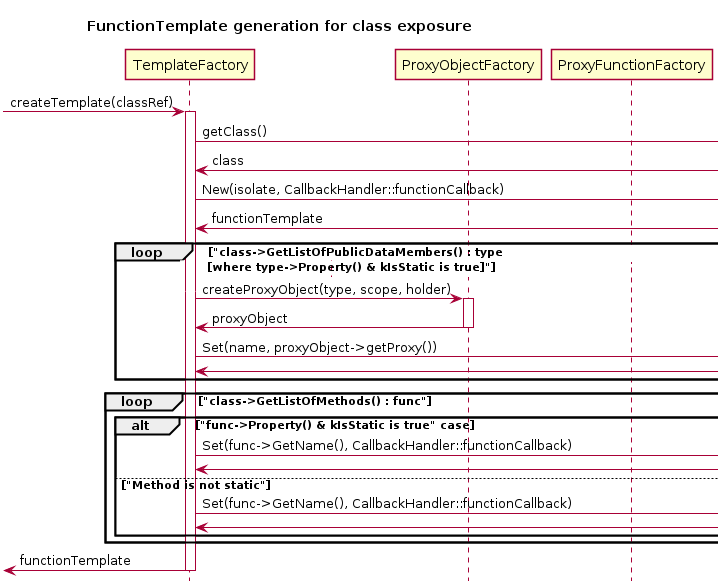
\includegraphics[width=16cm]{./latex/resources/functionTemplateGenerateCrop.png}
	\caption{function template creation (full diagram in appendix)}
\end{figure}

\chapter{TemplateCache}
describe class TemplateCache here
\section{contains}
\begin{longtable}{p{3cm} @{\hskip 1cm} p{12cm}}
 \hline
\textit{Name} & \texttt{TemplateCache::contains(type: TClassRef)}\\
\hline
 \textit{Visibility} & public\\
\hline
\textit{Parameters} & \textit{type: TClassRef}\\
\hline
\textit{Return value} & \textbf{ bool} describe return value\\
  \hline
 \textit{behavior} & describe beahviour \\
\hline
\end{longtable} \pagebreak
 \section{get}
\begin{longtable}{p{3cm} @{\hskip 1cm} p{12cm}}
 \hline
\textit{Name} & \texttt{TemplateCache::get(type: TClassRef)}\\
\hline
 \textit{Visibility} & public\\
\hline
\textit{Parameters} & \textit{type: TClassRef}\\
\hline
\textit{Return value} & \textbf{ Local<FunctionTemplate>} describe return value\\
  \hline
 \textit{behavior} & describe beahviour \\
\hline
\end{longtable} \pagebreak
 \section{store}
\begin{longtable}{p{3cm} @{\hskip 1cm} p{12cm}}
 \hline
\textit{Name} & \texttt{TemplateCache::store(type: TClassRef, tpl: Local<FunctionTemplate>)}\\
\hline
 \textit{Visibility} & public\\
\hline
\textit{Parameters} & \textit{type: TClassRef, tpl: Local<FunctionTemplate>}\\
\hline
\textit{Return value} & \textbf{none}\\
  \hline
 \textit{behavior} & describe beahviour \\
\hline
\end{longtable} \pagebreak
 
\chapter{ProxyFunctionFactory}
describe class ProxyFunctionFactory here
\section{ProxyFunctionFactory}
\begin{longtable}{p{3cm} @{\hskip 1cm} p{12cm}}
 \hline
\textit{Name} & \texttt{ProxyFunctionFactory::ProxyFunctionFactory()}\\
\hline
 \textit{Visibility} & public\\
\hline
\textit{Parameters} & \textit{none}\\
\hline
\textit{Return value} & \textbf{ <<constructor>>} describe return value\\
  \hline
 \textit{behavior} & describe beahviour \\
\hline
\end{longtable} \pagebreak
 \section{createProxyFunction}
\begin{longtable}{p{3cm} @{\hskip 1cm} p{12cm}}
 \hline
\textit{Name} & \texttt{ProxyFunctionFactory::createProxyFunction(function: TFunction, scope: TClassRef)}\\
\hline
 \textit{Visibility} & public\\
\hline
\textit{Parameters} & \textit{function: TFunction, scope: TClassRef}\\
\hline
\textit{Return value} & \textbf{ ProxyFunciton} describe return value\\
  \hline
 \textit{behavior} & describe beahviour \\
\hline
\end{longtable} \pagebreak
 \section{fromArgs}
\begin{longtable}{p{3cm} @{\hskip 1cm} p{12cm}}
 \hline
\textit{Name} & \texttt{ProxyFunctionFactory::fromArgs(name: string, scope: TClassRef, args: FunctionCallbackInfo)}\\
\hline
 \textit{Visibility} & public\\
\hline
\textit{Parameters} & \textit{name: string, scope: TClassRef, args: FunctionCallbackInfo}\\
\hline
\textit{Return value} & \textbf{ ProxyFunction} describe return value\\
  \hline
 \textit{behavior} & describe beahviour \\
\hline
\end{longtable} \pagebreak
 
\chapter{ProxyFunction}
describe class ProxyFunction here
\section{getCallFunc}
\begin{longtable}{p{3cm} @{\hskip 1cm} p{12cm}}
 \hline
\textit{Name} & \texttt{ProxyFunction::getCallFunc(method: TFunction*)}\\
\hline
 \textit{Visibility} & public\\
\hline
\textit{Parameters} & \textit{method: TFunction*}\\
\hline
\textit{Return value} & \textbf{ CallFunc*} describe return value\\
  \hline
 \textit{behavior} & describe beahviour \\
\hline
\end{longtable} \pagebreak
 \section{getMethodsFromName}
\begin{longtable}{p{3cm} @{\hskip 1cm} p{12cm}}
 \hline
\textit{Name} & \texttt{ProxyFunction::getMethodsFromName(scope: TClassRef, name: string)}\\
\hline
 \textit{Visibility} & public\\
\hline
\textit{Parameters} & \textit{scope: TClassRef, name: string}\\
\hline
\textit{Return value} & \textbf{ vector<TFunction*>} describe return value\\
  \hline
 \textit{behavior} & describe beahviour \\
\hline
\end{longtable} \pagebreak
 \section{ProxyFunction}
\begin{longtable}{p{3cm} @{\hskip 1cm} p{12cm}}
 \hline
\textit{Name} & \texttt{ProxyFunction::ProxyFunction(address: void*, function: TFunction, scope: TClassRef)}\\
\hline
 \textit{Visibility} & public\\
\hline
\textit{Parameters} & \textit{address: void*, function: TFunction, scope: TClassRef}\\
\hline
\textit{Return value} & \textbf{ <<constructor>>} describe return value\\
  \hline
 \textit{behavior} & describe beahviour \\
\hline
\end{longtable} \pagebreak
 \section{getType}
\begin{longtable}{p{3cm} @{\hskip 1cm} p{12cm}}
 \hline
\textit{Name} & \texttt{ProxyFunction::getType()}\\
\hline
 \textit{Visibility} & public\\
\hline
\textit{Parameters} & \textit{none}\\
\hline
\textit{Return value} & \textbf{ TFunction} describe return value\\
  \hline
 \textit{behavior} & describe beahviour \\
\hline
\end{longtable} \pagebreak
 \section{validateArgs}
\begin{longtable}{p{3cm} @{\hskip 1cm} p{12cm}}
 \hline
\textit{Name} & \texttt{ProxyFunction::validateArgs(args: FunctionCallbackInfo)}\\
\hline
 \textit{Visibility} & public\\
\hline
\textit{Parameters} & \textit{args: FunctionCallbackInfo}\\
\hline
\textit{Return value} & \textbf{ ProxyObject[]} describe return value\\
  \hline
 \textit{behavior} & describe beahviour \\
\hline
\end{longtable} \pagebreak
 \section{call}
\begin{longtable}{p{3cm} @{\hskip 1cm} p{12cm}}
 \hline
\textit{Name} & \texttt{ProxyFunction::call(args: ProxyObject[])}\\
\hline
 \textit{Visibility} & public\\
\hline
\textit{Parameters} & \textit{args: ProxyObject[]}\\
\hline
\textit{Return value} & \textbf{ ProxyObject} describe return value\\
  \hline
 \textit{behavior} & describe beahviour \\
\hline
\end{longtable} \pagebreak
 
\chapter{ProxyObjectFactory}
describe class ProxyObjectFactory here
\section{createProxyObject}
\begin{longtable}{p{3cm} @{\hskip 1cm} p{12cm}}
 \hline
\textit{Name} & \texttt{ProxyObjectFactory::createProxyObject(type: TDataMember, scope: TClassRef, holder: ProxyObject)}\\
\hline
 \textit{Visibility} & public\\
\hline
\textit{Parameters} & \textit{type: TDataMember, scope: TClassRef, holder: ProxyObject}\\
\hline
\textit{Return value} & \textbf{ ProxyObject} describe return value\\
  \hline
 \textit{behavior} & describe beahviour \\
\hline
\end{longtable} \pagebreak
 
\chapter{ProxyObject}
ProxyObject is an interace defining the following abstract methods:
\section{isScalar}
\begin{longtable}{p{3cm} @{\hskip 1cm} p{12cm}}
  \hline
  \textit{Name} & \texttt{ProxyObject::isScalar())} \\
  \hline
  \textit{Visibility} & Public abstract \\
  \hline
  \textit{Parameters} & \textit{none} \\
  \hline
  \textit{Return value} & \textbf{bool} true: The object is scalar, no recursion is needed to create a ROOT/v8 representation \\
  \hline
  \textit{behavior} & This is usually just a return statement, as String, Number, Bool, ... ProxyObjects will always handle scalar data and ObjectProxyObjets will be the only non scalar ProxyObjects (and will therefor return false) \\
  \hline
\end{longtable}
\section{getV8Handle}
\begin{longtable}{p{3cm} @{\hskip 1cm} p{12cm}}
  \hline
  \textit{Name} & \texttt{ProxyObject::getV8Handle())} \\
  \hline
  \textit{Visibility} & Public abstract \\
  \hline
  \textit{Parameters} & \textit{none} \\
  \hline
  \textit{Return value} & \textbf{v8::Handle} A Handle will be generated continaing the data, used to initialize the ProxyObject. \\
  \hline
  \textit{behavior} & This highly depends on the obecjt's type scalar types might just call a constructor and return the result, ObjectProxyObjects will need to step down all through the objects children. \\
  \hline
\end{longtable}

\chapter{FunctionHelper.tex}
describe class FunctionHelper.tex here
\section{GetCallFunc}
\begin{longtable}{p{3cm} @{\hskip 1cm} p{12cm}}
 \hline
\textit{Name} & \texttt{FunctionHelper.tex::GetCallFunc(method: TCppMethod)}\\
\hline
 \textit{Visibility} & public\\
\hline
\textit{Parameters} & \textit{method: TCppMethod}\\
\hline
\textit{Return value} & \textbf{ CallFunc*} describe return value\\
  \hline
 \textit{behavior} & describe beahviour \\
\hline
\end{longtable} \pagebreak
 \section{copyArgs}
\begin{longtable}{p{3cm} @{\hskip 1cm} p{12cm}}
 \hline
\textit{Name} & \texttt{FunctionHelper.tex::copyArgs(args: void*, vargs: void**)}\\
\hline
 \textit{Visibility} & public\\
\hline
\textit{Parameters} & \textit{args: void*, vargs: void**}\\
\hline
\textit{Return value} & \textbf{ void} describe return value\\
  \hline
 \textit{behavior} & describe beahviour \\
\hline
\end{longtable} \pagebreak
 \section{FastCall}
\begin{longtable}{p{3cm} @{\hskip 1cm} p{12cm}}
 \hline
\textit{Name} & \texttt{FunctionHelper.tex::FastCall(method: TCppMethod, args: void*, self: void*, result: void*)}\\
\hline
 \textit{Visibility} & public\\
\hline
\textit{Parameters} & \textit{method: TCppMethod, args: void*, self: void*, result: void*}\\
\hline
\textit{Return value} & \textbf{ bool} describe return value\\
  \hline
 \textit{behavior} & describe beahviour \\
\hline
\end{longtable} \pagebreak
 \section{CallV}
\begin{longtable}{p{3cm} @{\hskip 1cm} p{12cm}}
 \hline
\textit{Name} & \texttt{FunctionHelper.tex::CallV(method: TCppMethod, self: TCppObject, args: void*)}\\
\hline
 \textit{Visibility} & public\\
\hline
\textit{Parameters} & \textit{method: TCppMethod, self: TCppObject, args: void*}\\
\hline
\textit{Return value} & \textbf{ void} describe return value\\
  \hline
 \textit{behavior} & describe beahviour \\
\hline
\end{longtable} \pagebreak
 \section{CallR}
\begin{longtable}{p{3cm} @{\hskip 1cm} p{12cm}}
 \hline
\textit{Name} & \texttt{FunctionHelper.tex::CallR(method: TCppMethod, self: TCppObject, args: void*)}\\
\hline
 \textit{Visibility} & public\\
\hline
\textit{Parameters} & \textit{method: TCppMethod, self: TCppObject, args: void*}\\
\hline
\textit{Return value} & \textbf{ void*} describe return value\\
  \hline
 \textit{behavior} & describe beahviour \\
\hline
\end{longtable} \pagebreak
 \section{CallS}
\begin{longtable}{p{3cm} @{\hskip 1cm} p{12cm}}
 \hline
\textit{Name} & \texttt{FunctionHelper.tex::CallS(method: TCppMethod, self: TCppObject, args: void*)}\\
\hline
 \textit{Visibility} & public\\
\hline
\textit{Parameters} & \textit{method: TCppMethod, self: TCppObject, args: void*}\\
\hline
\textit{Return value} & \textbf{ Char*} describe return value\\
  \hline
 \textit{behavior} & describe beahviour \\
\hline
\end{longtable} \pagebreak
 \section{CallO}
\begin{longtable}{p{3cm} @{\hskip 1cm} p{12cm}}
 \hline
\textit{Name} & \texttt{FunctionHelper.tex::CallO(method: TCppMethod, self: TCppObject, args: void*, resultype: TCppType)}\\
\hline
 \textit{Visibility} & public\\
\hline
\textit{Parameters} & \textit{method: TCppMethod, self: TCppObject, args: void*, resultype: TCppType}\\
\hline
\textit{Return value} & \textbf{ TCppObject} describe return value\\
  \hline
 \textit{behavior} & describe beahviour \\
\hline
\end{longtable} \pagebreak
 \section{CallConstructor}
\begin{longtable}{p{3cm} @{\hskip 1cm} p{12cm}}
 \hline
\textit{Name} & \texttt{FunctionHelper.tex::CallConstructor(method: TCppMethod, klass: TCppType, args: void*)}\\
\hline
 \textit{Visibility} & public\\
\hline
\textit{Parameters} & \textit{method: TCppMethod, klass: TCppType, args: void*}\\
\hline
\textit{Return value} & \textbf{ TCppObject} describe return value\\
  \hline
 \textit{behavior} & describe beahviour \\
\hline
\end{longtable} \pagebreak
 \section{CallDestructor}
\begin{longtable}{p{3cm} @{\hskip 1cm} p{12cm}}
 \hline
\textit{Name} & \texttt{FunctionHelper.tex::CallDestructor(type: TCppType, self: TCppObject)}\\
\hline
 \textit{Visibility} & public\\
\hline
\textit{Parameters} & \textit{type: TCppType, self: TCppObject}\\
\hline
\textit{Return value} & \textbf{ void} describe return value\\
  \hline
 \textit{behavior} & describe beahviour \\
\hline
\end{longtable} \pagebreak
 \section{IsConstructor}
\begin{longtable}{p{3cm} @{\hskip 1cm} p{12cm}}
 \hline
\textit{Name} & \texttt{FunctionHelper.tex::IsConstructor(method: TCppMethod)}\\
\hline
 \textit{Visibility} & public\\
\hline
\textit{Parameters} & \textit{method: TCppMethod}\\
\hline
\textit{Return value} & \textbf{ bool} describe return value\\
  \hline
 \textit{behavior} & describe beahviour \\
\hline
\end{longtable} \pagebreak
 \section{IsPublicMethod}
\begin{longtable}{p{3cm} @{\hskip 1cm} p{12cm}}
 \hline
\textit{Name} & \texttt{FunctionHelper.tex::IsPublicMethod(method: TCppMethod)}\\
\hline
 \textit{Visibility} & public\\
\hline
\textit{Parameters} & \textit{method: TCppMethod}\\
\hline
\textit{Return value} & \textbf{ bool} describe return value\\
  \hline
 \textit{behavior} & describe beahviour \\
\hline
\end{longtable} \pagebreak
 \section{IsStaticMethod}
\begin{longtable}{p{3cm} @{\hskip 1cm} p{12cm}}
 \hline
\textit{Name} & \texttt{FunctionHelper.tex::IsStaticMethod(method: TCppMethod)}\\
\hline
 \textit{Visibility} & public\\
\hline
\textit{Parameters} & \textit{method: TCppMethod}\\
\hline
\textit{Return value} & \textbf{ bool} describe return value\\
  \hline
 \textit{behavior} & describe beahviour \\
\hline
\end{longtable} \pagebreak
 \section{IsConstMethod}
\begin{longtable}{p{3cm} @{\hskip 1cm} p{12cm}}
 \hline
\textit{Name} & \texttt{FunctionHelper.tex::IsConstMethod(method: TCppMethod)}\\
\hline
 \textit{Visibility} & public\\
\hline
\textit{Parameters} & \textit{method: TCppMethod}\\
\hline
\textit{Return value} & \textbf{ bool} describe return value\\
  \hline
 \textit{behavior} & describe beahviour \\
\hline
\end{longtable} \pagebreak
 \section{IsMethodTemplate}
\begin{longtable}{p{3cm} @{\hskip 1cm} p{12cm}}
 \hline
\textit{Name} & \texttt{FunctionHelper.tex::IsMethodTemplate(method: TCppMethod)}\\
\hline
 \textit{Visibility} & public\\
\hline
\textit{Parameters} & \textit{method: TCppMethod}\\
\hline
\textit{Return value} & \textbf{ bool} describe return value\\
  \hline
 \textit{behavior} & describe beahviour \\
\hline
\end{longtable} \pagebreak
 \section{GetMethodNumTemplateArgs}
\begin{longtable}{p{3cm} @{\hskip 1cm} p{12cm}}
 \hline
\textit{Name} & \texttt{FunctionHelper.tex::GetMethodNumTemplateArgs(scope: TCppScope, imeth: TCppIndex)}\\
\hline
 \textit{Visibility} & public\\
\hline
\textit{Parameters} & \textit{scope: TCppScope, imeth: TCppIndex}\\
\hline
\textit{Return value} & \textbf{ TCppIndex} describe return value\\
  \hline
 \textit{behavior} & describe beahviour \\
\hline
\end{longtable} \pagebreak
 \section{GetMethodTemplateArgName}
\begin{longtable}{p{3cm} @{\hskip 1cm} p{12cm}}
 \hline
\textit{Name} & \texttt{FunctionHelper.tex::GetMethodTemplateArgName(scope: TCppScope, imeth: TCppIndex, iarg: TCppIndex)}\\
\hline
 \textit{Visibility} & public\\
\hline
\textit{Parameters} & \textit{scope: TCppScope, imeth: TCppIndex, iarg: TCppIndex}\\
\hline
\textit{Return value} & \textbf{ string} describe return value\\
  \hline
 \textit{behavior} & describe beahviour \\
\hline
\end{longtable} \pagebreak
 \section{GetNumMethods}
\begin{longtable}{p{3cm} @{\hskip 1cm} p{12cm}}
 \hline
\textit{Name} & \texttt{FunctionHelper.tex::GetNumMethods(scope: TCppScope)}\\
\hline
 \textit{Visibility} & public\\
\hline
\textit{Parameters} & \textit{scope: TCppScope}\\
\hline
\textit{Return value} & \textbf{ TCppIndex} describe return value\\
  \hline
 \textit{behavior} & describe beahviour \\
\hline
\end{longtable} \pagebreak
 \section{GetMethodIndexAt}
\begin{longtable}{p{3cm} @{\hskip 1cm} p{12cm}}
 \hline
\textit{Name} & \texttt{FunctionHelper.tex::GetMethodIndexAt(scope: TCppScope, imeth: TCppIndex)}\\
\hline
 \textit{Visibility} & public\\
\hline
\textit{Parameters} & \textit{scope: TCppScope, imeth: TCppIndex}\\
\hline
\textit{Return value} & \textbf{ TCppIndex} describe return value\\
  \hline
 \textit{behavior} & describe beahviour \\
\hline
\end{longtable} \pagebreak
 \section{GetMethodsFromName}
\begin{longtable}{p{3cm} @{\hskip 1cm} p{12cm}}
 \hline
\textit{Name} & \texttt{FunctionHelper.tex::GetMethodsFromName(scope: TCppScope, name: string)}\\
\hline
 \textit{Visibility} & public\\
\hline
\textit{Parameters} & \textit{scope: TCppScope, name: string}\\
\hline
\textit{Return value} & \textbf{ vector<TCppMethod>} describe return value\\
  \hline
 \textit{behavior} & describe beahviour \\
\hline
\end{longtable} \pagebreak
 \section{GetMethod}
\begin{longtable}{p{3cm} @{\hskip 1cm} p{12cm}}
 \hline
\textit{Name} & \texttt{FunctionHelper.tex::GetMethod(scope: TCppScope, imeth: TCppIndex)}\\
\hline
 \textit{Visibility} & public\\
\hline
\textit{Parameters} & \textit{scope: TCppScope, imeth: TCppIndex}\\
\hline
\textit{Return value} & \textbf{ TCppMethod} describe return value\\
  \hline
 \textit{behavior} & describe beahviour \\
\hline
\end{longtable} \pagebreak
 \section{GetMethodName}
\begin{longtable}{p{3cm} @{\hskip 1cm} p{12cm}}
 \hline
\textit{Name} & \texttt{FunctionHelper.tex::GetMethodName(method: TCppMethod)}\\
\hline
 \textit{Visibility} & public\\
\hline
\textit{Parameters} & \textit{method: TCppMethod}\\
\hline
\textit{Return value} & \textbf{ string} describe return value\\
  \hline
 \textit{behavior} & describe beahviour \\
\hline
\end{longtable} \pagebreak
 \section{GetMethodResultType}
\begin{longtable}{p{3cm} @{\hskip 1cm} p{12cm}}
 \hline
\textit{Name} & \texttt{FunctionHelper.tex::GetMethodResultType(method: TCppMethod)}\\
\hline
 \textit{Visibility} & public\\
\hline
\textit{Parameters} & \textit{method: TCppMethod}\\
\hline
\textit{Return value} & \textbf{ string} describe return value\\
  \hline
 \textit{behavior} & describe beahviour \\
\hline
\end{longtable} \pagebreak
 \section{GetMethodNumArgs}
\begin{longtable}{p{3cm} @{\hskip 1cm} p{12cm}}
 \hline
\textit{Name} & \texttt{FunctionHelper.tex::GetMethodNumArgs(method: TCppMethod)}\\
\hline
 \textit{Visibility} & public\\
\hline
\textit{Parameters} & \textit{method: TCppMethod}\\
\hline
\textit{Return value} & \textbf{ TCppIndex} describe return value\\
  \hline
 \textit{behavior} & describe beahviour \\
\hline
\end{longtable} \pagebreak
 \section{GetMethodReqArgs}
\begin{longtable}{p{3cm} @{\hskip 1cm} p{12cm}}
 \hline
\textit{Name} & \texttt{FunctionHelper.tex::GetMethodReqArgs(method: TCppMethod)}\\
\hline
 \textit{Visibility} & public\\
\hline
\textit{Parameters} & \textit{method: TCppMethod}\\
\hline
\textit{Return value} & \textbf{ TCppIndex} describe return value\\
  \hline
 \textit{behavior} & describe beahviour \\
\hline
\end{longtable} \pagebreak
 \section{GetMethodArgName}
\begin{longtable}{p{3cm} @{\hskip 1cm} p{12cm}}
 \hline
\textit{Name} & \texttt{FunctionHelper.tex::GetMethodArgName(method: TCppMethod, iarg: int)}\\
\hline
 \textit{Visibility} & public\\
\hline
\textit{Parameters} & \textit{method: TCppMethod, iarg: int}\\
\hline
\textit{Return value} & \textbf{ string} describe return value\\
  \hline
 \textit{behavior} & describe beahviour \\
\hline
\end{longtable} \pagebreak
 \section{GetMethodArgType}
\begin{longtable}{p{3cm} @{\hskip 1cm} p{12cm}}
 \hline
\textit{Name} & \texttt{FunctionHelper.tex::GetMethodArgType(method: TCppMethod, iarg: int)}\\
\hline
 \textit{Visibility} & public\\
\hline
\textit{Parameters} & \textit{method: TCppMethod, iarg: int}\\
\hline
\textit{Return value} & \textbf{ string} describe return value\\
  \hline
 \textit{behavior} & describe beahviour \\
\hline
\end{longtable} \pagebreak
 \section{GetMethodArgDefault}
\begin{longtable}{p{3cm} @{\hskip 1cm} p{12cm}}
 \hline
\textit{Name} & \texttt{FunctionHelper.tex::GetMethodArgDefault(method: TCppMethod, iarg: int)}\\
\hline
 \textit{Visibility} & public\\
\hline
\textit{Parameters} & \textit{method: TCppMethod, iarg: int}\\
\hline
\textit{Return value} & \textbf{ string} describe return value\\
  \hline
 \textit{behavior} & describe beahviour \\
\hline
\end{longtable} \pagebreak
 \section{GetMethodSignature}
\begin{longtable}{p{3cm} @{\hskip 1cm} p{12cm}}
 \hline
\textit{Name} & \texttt{FunctionHelper.tex::GetMethodSignature(scope: TCppScope, imeth: TCppIndex)}\\
\hline
 \textit{Visibility} & public\\
\hline
\textit{Parameters} & \textit{scope: TCppScope, imeth: TCppIndex}\\
\hline
\textit{Return value} & \textbf{ string} describe return value\\
  \hline
 \textit{behavior} & describe beahviour \\
\hline
\end{longtable} \pagebreak
 
\chapter{ClassHelper}
describe class ClassHelper here
\section{IsNamespace}
\begin{longtable}{p{3cm} @{\hskip 1cm} p{12cm}}
 \hline
\textit{Name} & \texttt{ClassHelper::IsNamespace(scope: TCppScope)}\\
\hline
 \textit{Visibility} & public\\
\hline
\textit{Parameters} & \textit{scope: TCppScope}\\
\hline
\textit{Return value} & \textbf{ bool} Returns a boolean which checks if the scope represents a namespace.\\
  \hline
 \textit{behavior} & Checks if scope represents a namespace. \\
\hline
\end{longtable} \pagebreak
 \section{IsAbstract}
\begin{longtable}{p{3cm} @{\hskip 1cm} p{12cm}}
 \hline
\textit{Name} & \texttt{ClassHelper::IsAbstract(klass: TCppType)}\\
\hline
 \textit{Visibility} & public\\
\hline
\textit{Parameters} & \textit{klass: TCppType}\\
\hline
\textit{Return value} & \textbf{ bool} describe return value\\
  \hline
 \textit{behavior} & Checks if klass is an abstract class, and hence can be instantiated or not. \\
\hline
\end{longtable} \pagebreak
 \section{IsEnum}
\begin{longtable}{p{3cm} @{\hskip 1cm} p{12cm}}
 \hline
\textit{Name} & \texttt{ClassHelper::IsEnum(typename: string)}\\
\hline
 \textit{Visibility} & public\\
\hline
\textit{Parameters} & \textit{typename: string}\\
\hline
\textit{Return value} & \textbf{ bool} describe return value\\
  \hline
 \textit{behavior} & Checks if string represents a enum. \\
\hline
\end{longtable} \pagebreak
 \section{IsStruct}
\begin{longtable}{p{3cm} @{\hskip 1cm} p{12cm}}
 \hline
\textit{Name} & \texttt{ClassHelper::IsStruct(typename: string)}\\
\hline
 \textit{Visibility} & public\\
\hline
\textit{Parameters} & \textit{typename: string}\\
\hline
\textit{Return value} & \textbf{ bool} describe return value\\
  \hline
 \textit{behavior} & Checks if string is a struct datatype. \\
\hline
\end{longtable} \pagebreak
 \section{GetFinalName}
\begin{longtable}{p{3cm} @{\hskip 1cm} p{12cm}}
 \hline
\textit{Name} & \texttt{ClassHelper::GetFinalName(klass: TCppType)}\\
\hline
 \textit{Visibility} & public\\
\hline
\textit{Parameters} & \textit{klass: TCppType}\\
\hline
\textit{Return value} & \textbf{ string} describe return value\\
  \hline
 \textit{behavior} & describe beahviour \\
\hline
\end{longtable} \pagebreak
 \section{GetScopedFinalName}
\begin{longtable}{p{3cm} @{\hskip 1cm} p{12cm}}
 \hline
\textit{Name} & \texttt{ClassHelper::GetScopedFinalName(klass: TCppType)}\\
\hline
 \textit{Visibility} & public\\
\hline
\textit{Parameters} & \textit{klass: TCppType}\\
\hline
\textit{Return value} & \textbf{ string} describe return value\\
  \hline
 \textit{behavior} & describe beahviour \\
\hline
\end{longtable} \pagebreak
 \section{GetNumBases}
\begin{longtable}{p{3cm} @{\hskip 1cm} p{12cm}}
 \hline
\textit{Name} & \texttt{ClassHelper::GetNumBases(klass: TCppType)}\\
\hline
 \textit{Visibility} & public\\
\hline
\textit{Parameters} & \textit{klass: TCppType}\\
\hline
\textit{Return value} & \textbf{ TCppIndex} describe return value\\
  \hline
 \textit{behavior} & Returns the number of base classes this class contains. \\
\hline
\end{longtable} \pagebreak
 \section{GetBaseName}
\begin{longtable}{p{3cm} @{\hskip 1cm} p{12cm}}
 \hline
\textit{Name} & \texttt{ClassHelper::GetBaseName(klass: TCppType, ibase: TCppIndex)}\\
\hline
 \textit{Visibility} & public\\
\hline
\textit{Parameters} & \textit{klass: TCppType, ibase: TCppIndex}\\
\hline
\textit{Return value} & \textbf{ string} describe return value\\
  \hline
 \textit{behavior} & describe beahviour \\
\hline
\end{longtable} \pagebreak
 \section{IsSubtype}
\begin{longtable}{p{3cm} @{\hskip 1cm} p{12cm}}
 \hline
\textit{Name} & \texttt{ClassHelper::IsSubtype(derived: TCppType, base: TCppType)}\\
\hline
 \textit{Visibility} & public\\
\hline
\textit{Parameters} & \textit{derived: TCppType, base: TCppType}\\
\hline
\textit{Return value} & \textbf{ bool} describe return value\\
  \hline
 \textit{behavior} & describe beahviour \\
\hline
\end{longtable} \pagebreak
 \section{GetNumDatamembers}
\begin{longtable}{p{3cm} @{\hskip 1cm} p{12cm}}
 \hline
\textit{Name} & \texttt{ClassHelper::GetNumDatamembers(scope: TCppScope)}\\
\hline
 \textit{Visibility} & public\\
\hline
\textit{Parameters} & \textit{scope: TCppScope}\\
\hline
\textit{Return value} & \textbf{ TCppIndex} describe return value\\
  \hline
 \textit{behavior} & describe beahviour \\
\hline
\end{longtable} \pagebreak
 \section{GetDatamemberName}
\begin{longtable}{p{3cm} @{\hskip 1cm} p{12cm}}
 \hline
\textit{Name} & \texttt{ClassHelper::GetDatamemberName(scope: TCppScope, idata: TCppIndex)}\\
\hline
 \textit{Visibility} & public\\
\hline
\textit{Parameters} & \textit{scope: TCppScope, idata: TCppIndex}\\
\hline
\textit{Return value} & \textbf{ string} describe return value\\
  \hline
 \textit{behavior} & describe beahviour \\
\hline
\end{longtable} \pagebreak
 \section{GetDatamemberType}
\begin{longtable}{p{3cm} @{\hskip 1cm} p{12cm}}
 \hline
\textit{Name} & \texttt{ClassHelper::GetDatamemberType(scope: TCppScope, idata: TCppIndex)}\\
\hline
 \textit{Visibility} & public\\
\hline
\textit{Parameters} & \textit{scope: TCppScope, idata: TCppIndex}\\
\hline
\textit{Return value} & \textbf{ string} describe return value\\
  \hline
 \textit{behavior} & describe beahviour \\
\hline
\end{longtable} \pagebreak
 \section{GetDatamemberOffset}
\begin{longtable}{p{3cm} @{\hskip 1cm} p{12cm}}
 \hline
\textit{Name} & \texttt{ClassHelper::GetDatamemberOffset(scope: TCppScope, idata: TCppIndex)}\\
\hline
 \textit{Visibility} & public\\
\hline
\textit{Parameters} & \textit{scope: TCppScope, idata: TCppIndex}\\
\hline
\textit{Return value} & \textbf{ ptrdiff} describe return value\\
  \hline
 \textit{behavior} & describe beahviour \\
\hline
\end{longtable} \pagebreak
 \section{GetDatamemberIndex}
\begin{longtable}{p{3cm} @{\hskip 1cm} p{12cm}}
 \hline
\textit{Name} & \texttt{ClassHelper::GetDatamemberIndex(scope: TCppScope, name: string)}\\
\hline
 \textit{Visibility} & public\\
\hline
\textit{Parameters} & \textit{scope: TCppScope, name: string}\\
\hline
\textit{Return value} & \textbf{ TCppIndex} describe return value\\
  \hline
 \textit{behavior} & describe beahviour \\
\hline
\end{longtable} \pagebreak
 \section{IsPublicData}
\begin{longtable}{p{3cm} @{\hskip 1cm} p{12cm}}
 \hline
\textit{Name} & \texttt{ClassHelper::IsPublicData(scope: TCppScope, idata: TCppIndex)}\\
\hline
 \textit{Visibility} & public\\
\hline
\textit{Parameters} & \textit{scope: TCppScope, idata: TCppIndex}\\
\hline
\textit{Return value} & \textbf{ bool} describe return value\\
  \hline
 \textit{behavior} & describe beahviour \\
\hline
\end{longtable} \pagebreak
 \section{IsStaticData}
\begin{longtable}{p{3cm} @{\hskip 1cm} p{12cm}}
 \hline
\textit{Name} & \texttt{ClassHelper::IsStaticData(scope: TCppScope, idata: TCppIndex)}\\
\hline
 \textit{Visibility} & public\\
\hline
\textit{Parameters} & \textit{scope: TCppScope, idata: TCppIndex}\\
\hline
\textit{Return value} & \textbf{ bool} describe return value\\
  \hline
 \textit{behavior} & describe beahviour \\
\hline
\end{longtable} \pagebreak
 \section{IsConstData}
\begin{longtable}{p{3cm} @{\hskip 1cm} p{12cm}}
 \hline
\textit{Name} & \texttt{ClassHelper::IsConstData(scope: TCppScope, idata: TCppIndex)}\\
\hline
 \textit{Visibility} & public\\
\hline
\textit{Parameters} & \textit{scope: TCppScope, idata: TCppIndex}\\
\hline
\textit{Return value} & \textbf{ bool} describe return value\\
  \hline
 \textit{behavior} & describe beahviour \\
\hline
\end{longtable} \pagebreak
 \section{IsEnumData}
\begin{longtable}{p{3cm} @{\hskip 1cm} p{12cm}}
 \hline
\textit{Name} & \texttt{ClassHelper::IsEnumData(scope: TCppScope, idata: TCppIndex)}\\
\hline
 \textit{Visibility} & public\\
\hline
\textit{Parameters} & \textit{scope: TCppScope, idata: TCppIndex}\\
\hline
\textit{Return value} & \textbf{ bool} describe return value\\
  \hline
 \textit{behavior} & describe beahviour \\
\hline
\end{longtable} \pagebreak
 \section{resolveAddress}
\begin{longtable}{p{3cm} @{\hskip 1cm} p{12cm}}
 \hline
\textit{Name} & \texttt{ClassHelper::resolveAddress(staticMember: TDataMember, clazz: TClassRef)}\\
\hline
 \textit{Visibility} & public\\
\hline
\textit{Parameters} & \textit{staticMember: TDataMember, clazz: TClassRef}\\
\hline
\textit{Return value} & \textbf{ void*} describe return value\\
  \hline
 \textit{behavior} & describe beahviour \\
\hline
\end{longtable} \pagebreak
 \section{resolveAddress}
\begin{longtable}{p{3cm} @{\hskip 1cm} p{12cm}}
 \hline
\textit{Name} & \texttt{ClassHelper::resolveAddress(staticMember: TDataMember, clazz: TClassRef)}\\
\hline
 \textit{Visibility} & public\\
\hline
\textit{Parameters} & \textit{staticMember: TDataMember, clazz: TClassRef}\\
\hline
\textit{Return value} & \textbf{ void*} describe return value\\
  \hline
 \textit{behavior} & describe beahviour \\
\hline
\end{longtable} \pagebreak
 
\end{document}
